\chapter{Lezione 13 - Cloud computing - I servizi}

Benvenuti a questa lezione parleremo del cloud computing, i servizi.
Gli argomenti che affronteremo sono i tipi di servizi erogati e le classi di consumatori che possono farne richiesta.

Argomenti trattati:

\FloatBarrier
\begin{figure}[H]
  \centering
  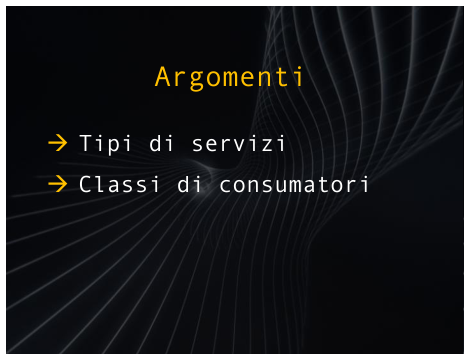
\includegraphics[width=0.50\textwidth,
                    trim=40 140 40 60, % L B R T
                    clip]
                    {images/Lez13_p01_fig_02}
  % \caption{Sommario}
  % \label{fig:Lez15_p06_fig_02}
\end{figure}
\FloatBarrier
\noindent


Abbiamo visto che questi due sono elementi costituenti del modello cloud computing.

\section{Tipi di servizi}

Mostreremo una rassegna di tutti i modelli di servizio per la gestione delle risorse disponibili offerti da questo modello di erogazione di risorse cloud computing.

\FloatBarrier
\begin{figure}[H]
  \centering
  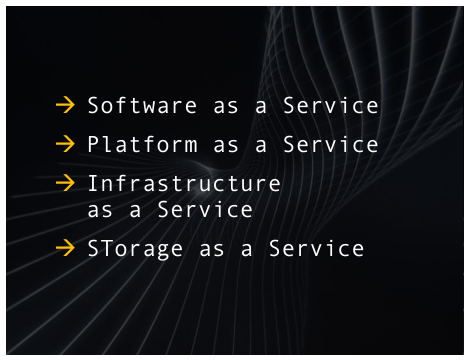
\includegraphics[width=0.50\textwidth,
                    trim=40 80 40 60, % L B R T
                    clip]
                    {images/Lez13_p01_fig_04}
  % \caption{Sommario}
  % \label{fig:Lez15_p06_fig_02}
\end{figure}
\FloatBarrier
\noindent

Software as a service.
Sinteticamente fa riferimento alla gestione di una applicazione completa.
Viene offerto un servizio di utenza finale a un'applicazione, non un ambiente di sviluppo, non un'infrastruttura su cui l'utente può installare ulteriori applicativi, ma proprio un'applicazione definita che viene offerta all'utente che ne fa richiesta.

In seguito vedremo platform as a service, che è l'offerta di servizio più aperta.
Si riferisce ad ambienti di sviluppo, ad ambienti offerti al cliente, in cui il cliente possa sviluppare una propria applicazione, possa lavorare per creare un proprio prodotto.
Quindi abbiamo a che fare con l'offerta di un ambiente di sviluppo, possibilmente.

Poi abbiamo infrastructure as a service.
Infrastructure as a service fa riferimento proprio all'offerta di un'infrastruttura hardware virtualizzata.
Quindi l'utente ha un'immagine del livello fisico di risorse utilizzabili con il massimo della possibilità di configurazione.

Poi vedremo storage as a service.
Fa riferimento a servizi per l'organizzazione di dati.
In genere sono servizi che offrono aree comuni per memorizzare file, quindi immagini di file system, in cui però, spesso, essendo aree condivise da un gruppo eventualmente ristretto di collaboratori, vengono forniti anche applicativi, strumenti, per la condivisione di questi file in applicazione, in offering per la possibilità di lavorare su questi dati, eventualmente su questi testi, in maniera multiutente, in maniera partecipata.

\FloatBarrier
\begin{figure}[H]
  \centering
  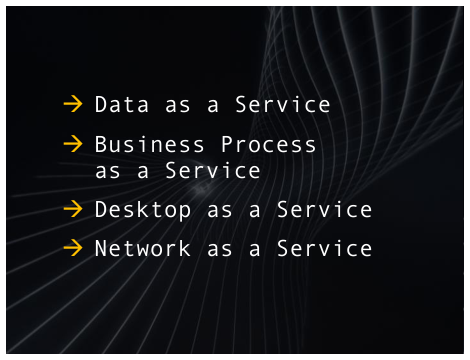
\includegraphics[width=0.50\textwidth,
                    trim=40 80 40 60, % L B R T
                    clip]
                    {images/Lez13_p01_fig_05}
  % \caption{Sommario}
  % \label{fig:Lez15_p06_fig_02}
\end{figure}
\FloatBarrier
\noindent

Vedremo poi Data as a service.
Accesso a archivi di dati eterogenei, servizi che vengono forniti spesso con interfacce, con applicativi, che permettono sia di organizzare questi dati, ma soprattutto di ricercarli e produrre dati, organizzazioni nuove di dati a valore aggiunto, con ulteriori specificità rispetto a quelle delle fonti primarie.

Business process as a service fa riferimento a una gamma di servizi a sistemi informativi aziendali, di tutti i tipi noti, di tutti i tipi disponibili, quindi accesso da utente aziendale a una applicazione, a un sistema piuttosto complesso.

Desktop as a service per l'utilizzo di desktop virtuali, per la condivisione di monitor, per attività collaborative, attività di gruppo.

Network as a service.
L'utente chiede la possibilità di collegamento alla rete, non specifica le risorse che saranno collegate, sarà lui stesso a sceglierle durante l'uso del servizio, ma chiede proprio un collegamento specifico a rete.
Quindi in questo caso sarà importante la larghezza di banda o la qualità, la protezione della connessione.

\subsection{Software as a Service SAAS}

\FloatBarrier
\begin{figure}[H]
  \centering
  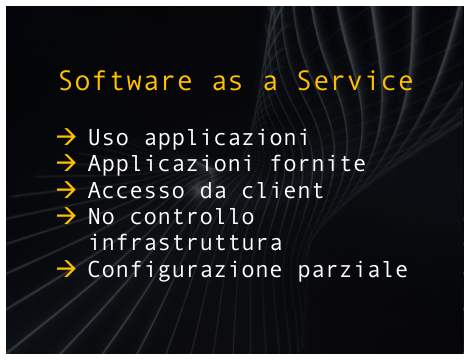
\includegraphics[width=0.50\textwidth,
                    trim=40 60 40 60, % L B R T
                    clip]
                    {images/Lez13_p01_fig_06}
  % \caption{Sommario}
  % \label{fig:Lez15_p06_fig_02}
\end{figure}
\FloatBarrier
\noindent

L'uso di applicazioni.
Abbiamo accennato che questo tipo di servizio offre applicazioni end user, offre applicazioni già sviluppate perché possano essere usufruite eventualmente in multiutenza.
Sono applicazioni fornite specificatamente dal provider del servizio, sono state sviluppate nel suo ambito o eventualmente da terzi, possono essere accedute da vari client.
In genere nel modello di erogazione di servizi cloud è lasciata libertà di client.

L'utente può collegarsi da un ampio spettro di client, siano leggeri, pesanti, standard, piuttosto che forniti specifici per il tipo di cloud stesso, client gestiti da applicazioni da app per mobile e così via.

L'utente non ha un controllo dell'infrastruttura sottostante, gli è fornito semplicemente il controllo dell'applicazione stessa, solo il livello di servizio richiesto è permesso all'utente.
L'utente in questo caso specifico può definire i parametri di configurazione dell'applicazione che gli è offerta.
La configurazione può essere parziale, dipendente dal livello di servizio richiesto, dal tipo di applicazione e dal tipo di accesso che è stato richiesto nel servizio stesso.

\FloatBarrier
\begin{figure}[H]
  \centering
  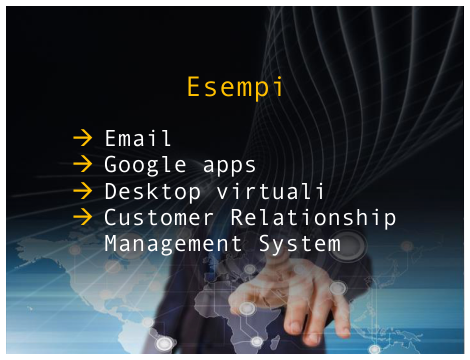
\includegraphics[width=0.50\textwidth,
                    trim=40 80 40 60, % L B R T
                    clip]
                    {images/Lez13_p02_fig_01}
  % \caption{Sommario}
  % \label{fig:Lez15_p06_fig_02}
\end{figure}
\FloatBarrier
\noindent

Alcuni esempi sono la gestione di caselle di posta elettronica, all'utente può essere chiesta la possibilità di utilizzare delle caselle piuttosto che di gestirle, ecco che gli verranno permessi accessi e configurazioni differenti da amministratori oppure solo di utenza per le proprie singole caselle.
Oppure Google Apps, vedremo in seguito che tipo di servizio rappresentano, vedremo un po' più nel dettaglio nelle prossime slide.

Altri esempi sono desktop virtuali, applicazioni specifiche che simulano un terminale per poter permettere a un gruppo di collaboratori di lavorare in maniera interattiva vedendo sullo stesso schermo il lavoro che stanno svolgendo, i dati che stanno producendo.

Customer Relationship Management System, quindi l'accesso anche a sistemi più complessi.
L'idea di questo modello di servizio è che l'utente si trovi davanti a un'applicazione finita per quanto complessa essa sia; non siamo nell'ambito dello sviluppo, non siamo nell'ambito dell'organizzazione di risorse, ma siamo proprio nell'ambito dell'uso di un'applicazione d'utente, applicazione finita.

\FloatBarrier
\begin{figure}[H]
  \centering
  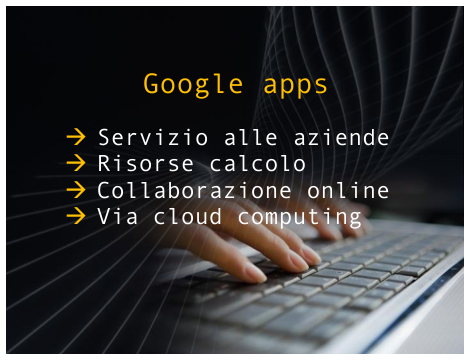
\includegraphics[width=0.50\textwidth,
                    trim=40 100 40 60, % L B R T
                    clip]
                    {images/Lez13_p02_fig_02}
  % \caption{Sommario}
  % \label{fig:Lez15_p06_fig_02}
\end{figure}
\FloatBarrier
\noindent

Vediamo cosa sono le Google Apps.
Sono un servizio dedicato alle aziende, un servizio di calcolo, un servizio che organizza servizi di calcolo, permette la collaborazione online, quindi l'utilizzo interattivo, l'utilizzo condiviso di queste risorse, attraverso il cloud computing, attraverso questo modello di erogazione di servizi che stiamo analizzando.

\FloatBarrier
\begin{figure}[H]
  \centering
  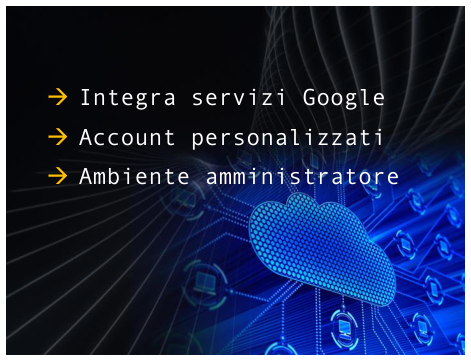
\includegraphics[width=0.50\textwidth,
                    trim=40 160 40 60, % L B R T
                    clip]
                    {images/Lez13_p02_fig_03}
  % \caption{Sommario}
  % \label{fig:Lez15_p06_fig_02}
\end{figure}
\FloatBarrier
\noindent

Queste Google Apps integrano servizi di Google e offrono accesso a servizi di Google raggruppati per specificità aziendale.
Un'azienda desidera l'accesso a questo tipo di servizi, le viene offerto un raggruppamento di questi servizi con interfaccia per il loro accesso, per il loro sfruttamento.
Vengono inoltre forniti account personalizzati, quindi l'utente può avere possibilità di accesso differenziato, accesso personalizzato per le proprie esigenze e per le proprie priorità di accesso.
L'utente può definire dei propri gruppi di utenze grazie anche alla possibilità di usufruire di un ambiente di amministratore per definire lui stesso il tipo di utente e le caratteristiche che ogni utente deve avere, quindi le funzionalità a cui ha accesso e quali sono i servizi a cui ha accesso.

\subsection{Platform as a Service}

\FloatBarrier
\begin{figure}[H]
  \centering
  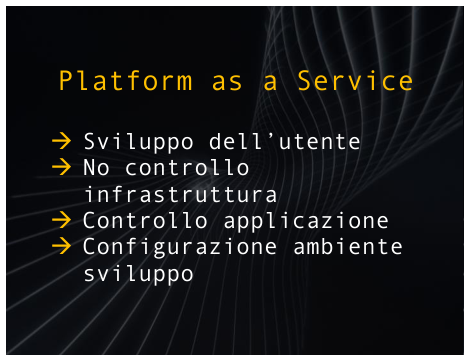
\includegraphics[width=0.50\textwidth,
                    trim=40 60 40 60, % L B R T
                    clip]
                    {images/Lez13_p02_fig_04}
  % \caption{Sommario}
  % \label{fig:Lez15_p06_fig_02}
\end{figure}
\FloatBarrier
\noindent

Il servizio successivo, il modello di servizio è platform as a service, ambiente di sviluppo dell'utente.
L'utente in questo caso non si trova davanti a un'applicazione, ma ha un ambiente applicativo in cui può sviluppare una propria applicazione.
L'utente deve sviluppare delle applicazioni ma non intende acquisire proprie risorse di calcolo che potrebbero richiedere l'acquisizione anche di ulteriore personale, di ulteriore competenze e non intende acquisire la licenza per l'ambiente di sviluppo.
Fa riferimento quindi all'erogazione di questo tipo di servizio, un ambiente di sviluppo offerto non come licenza d'uso ma come servizio a consumo.

In questo caso non è permesso il controllo dell'infrastruttura su cui è installato questo ambiente di sviluppo, ma all'utente viene permesso solo il controllo, la personalizzazione, la configurazione dell'ambiente di sviluppo e naturalmente dell'applicazione che lui stesso ha sviluppato.

L'utente ha la possibilità completa del controllo di quanto sviluppato in questo ambiente e la possibilità di configurare, di modificare l'ambiente di sviluppo, la platform che gli è stata offerta come servizio.

\FloatBarrier
\begin{figure}[H]
  \centering
  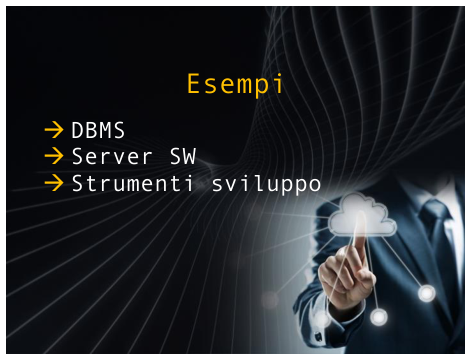
\includegraphics[width=0.50\textwidth,
                    trim=40 160 40 60, % L B R T
                    clip]
                    {images/Lez13_p02_fig_05}
  % \caption{Sommario}
  % \label{fig:Lez15_p06_fig_02}
\end{figure}
\FloatBarrier
\noindent

Un ambito di sviluppo di applicazioni per database management system in cui all'utente è fornito il sistema di gestione di una base di dati, ad esempio relazionale e la possibilità di sviluppare nuove interfacce o programmi di altro genere che peschino i dati, che accedano ai database offerti e possano creare una reportistica recuperando i dati.

Oppure server software in cui l'utente può sviluppare il proprio sito web, il proprio portale, piuttosto che installare un'altra propria applicazione.
Ad esempio, la offerta di un database management system per esempio online o un insieme di dati, quindi un archivio offerto in consultazione tramite web.
Oppure altri strumenti per lo sviluppo generale di applicazione, quindi ambiti per la programmazione in linguaggi di basso livello, anche LISP, Java, piuttosto che altri linguaggi.


\subsection{Infrastructure as a Service}

\FloatBarrier
\begin{figure}[H]
  \centering
  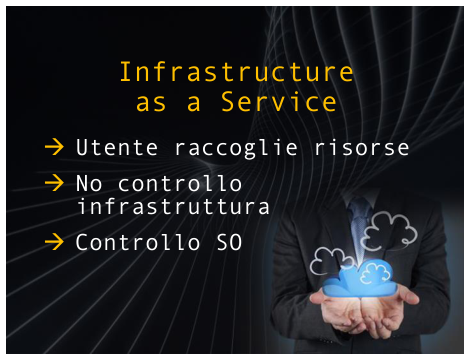
\includegraphics[width=0.50\textwidth,
                    trim=40 80 40 60, % L B R T
                    clip]
                    {images/Lez13_p02_fig_06}
  % \caption{Sommario}
  % \label{fig:Lez15_p06_fig_02}
\end{figure}
\FloatBarrier
\noindent

Un servizio generale verso il livello fisico è l'infrastructure as a service.
L'utente organizza le proprie risorse.
A livello fisico in quanto è proprio l'utente che definisce, seleziona quali sono le risorse che gli interessano e gli vengono presentati nella versione virtualizzata.

Potrà controllare il sistema operativo, piuttosto che a un sistema di archiviazione o di accesso alla rete, eventualmente potendo controllare un router o un firewall come sistemi di protezione.

Non è dato il controllo all'infrastruttura di base, se non parziale per il controllo dell'accesso alla rete, quindi l'eventuale firewall virtuale, che è il software che gli è offerto, oppure il controllo al sistema operativo che gli è stato offerto per la gestione delle risorse.

\FloatBarrier
\begin{figure}[H]
  \centering
  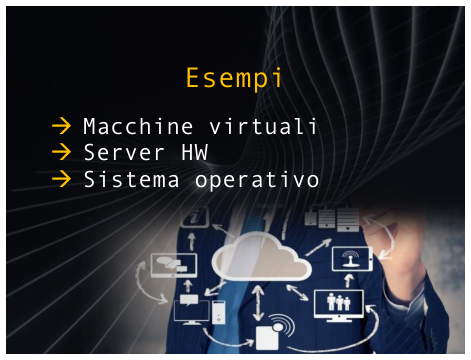
\includegraphics[width=0.50\textwidth,
                    trim=40 140 40 60, % L B R T
                    clip]
                    {images/Lez13_p03_fig_01}
  % \caption{Sommario}
  % \label{fig:Lez15_p06_fig_02}
\end{figure}
\FloatBarrier
\noindent

Alcuni esempi sono l'offerta di macchine virtuali all'utente, piuttosto che server hardware.

Server hardware vuol dire che viene offerta all'utente una macchina virtuale, proprio la virtualizzazione di un computer su cui potrà installare server software di qualsiasi tipo, che sia il server web, piuttosto che un server per la gestione di DBMS online, piuttosto che per gestirsi autonomamente il proprio server di posta senza usufruire dell'applicativo del fornitore per la posta elettronica, cioè della gestione di posta fornita dal provider.

Altro esempio è un sistema operativo specifico che ci viene fornito non in licenza d'uso ma a consumo come servizio.

\FloatBarrier
\begin{figure}[H]
  \centering
  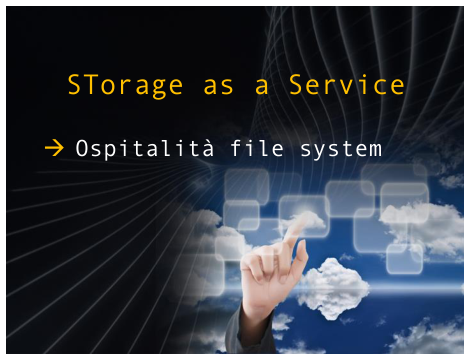
\includegraphics[width=0.50\textwidth,
                    trim=40 140 40 60, % L B R T
                    clip]
                    {images/Lez13_p03_fig_02}
  % \caption{Sommario}
  % \label{fig:Lez15_p06_fig_02}
\end{figure}
\FloatBarrier
\noindent

Un altro modello di servizio è storage as a service per l'ospitalità di file system.
Ce ne sono vari casi, sono molto utilizzati, offrono generalmente proprio un modello di organizzazione dei dati tipo file system accompagnato da possibilità di scegliere gli utenti con cui condividere, gestire gruppi d'accesso e eventualmente condividere con questi collaboratori il versioning delle modifiche che possono essere effettuate sui dati, eventualmente sui testi in questo file system o mandare messaggi autonomamente di notifica o di allerta.

\FloatBarrier
\begin{figure}[H]
  \centering
  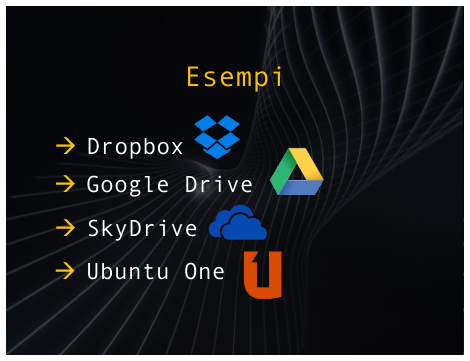
\includegraphics[width=0.50\textwidth,
                    trim=40 40 40 60, % L B R T
                    clip]
                    {images/Lez13_p03_fig_03}
  % \caption{Sommario}
  % \label{fig:Lez15_p06_fig_02}
\end{figure}
\FloatBarrier
\noindent

Alcuni esempi li conosciamo sono Dropbox, piuttosto che Google Drive per la condivisione e l'editing di condiviso di file, SkyDrive o Ubuntu One, è un quarto esempio ben noto.

\subsection{Data as a Service}

\FloatBarrier
\begin{figure}[H]
  \centering
  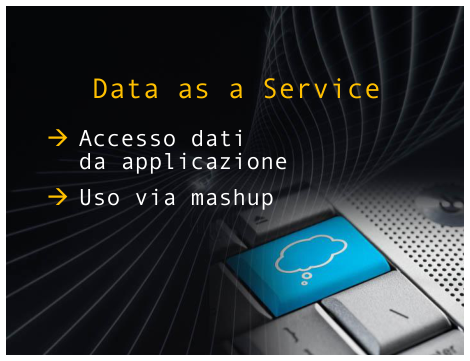
\includegraphics[width=0.50\textwidth,
                    trim=40 140 40 60, % L B R T
                    clip]
                    {images/Lez13_p03_fig_04}
  % \caption{Sommario}
  % \label{fig:Lez15_p06_fig_02}
\end{figure}
\FloatBarrier
\noindent

Che differenza c'è?
Ma in questo caso è offerto accesso a varie fonti di dati, a vari archivi, si presuppone che l'utente abbia necessità di integrare dati per produrre valore aggiunto, per produrre nuovi dati, integrare informazioni, per interpretarle, produrre nuova conoscenza, produrre nuovi documenti, attingendo a varie fonti selezionate.

\FloatBarrier
\begin{figure}[H]
  \centering
  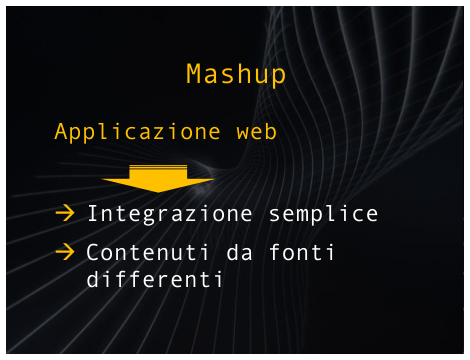
\includegraphics[width=0.50\textwidth,
                    trim=40 60 40 60, % L B R T
                    clip]
                    {images/Lez13_p03_fig_05}
  % \caption{Sommario}
  % \label{fig:Lez15_p06_fig_02}
\end{figure}
\FloatBarrier
\noindent

Quindi vengono forniti anche mashup; l'uso via mashup che sono applicazioni web per l'integrazione semplice di contenuti da fonti che sono differenti.

\FloatBarrier
\begin{figure}[H]
  \centering
  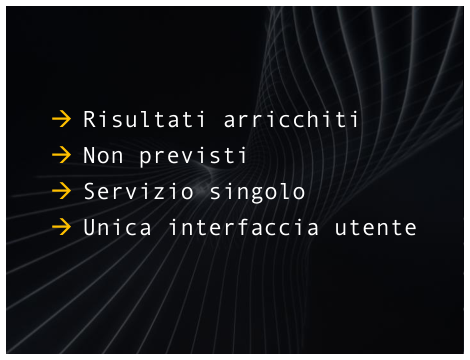
\includegraphics[width=0.50\textwidth,
                    trim=40 100 40 80, % L B R T
                    clip]
                    {images/Lez13_p03_fig_06}
  % \caption{Sommario}
  % \label{fig:Lez15_p06_fig_02}
\end{figure}
\FloatBarrier
\noindent

Utilizzano generalmente delle API, dell'Application Programming Interface, che permettono a questa interfaccia di mashup di selezionare le fonti, di accedere alle fonti, raccogliere i dati necessari e in maniera molto semplice selezionarli e produrre delle sintesi che puntano a produrre risultati arricchiti, risultati con valore aggiunto che non necessariamente erano previsti nelle fonti originarie.
Sostanzialmente si tratta di fornire delle interfacce che forniscano un servizio singolo all'utente di accesso a interfacce differenziate, interfacce che forniscono dati di formati e con metodi di accesso differenti, ma attraverso un'unica interfaccia utente.
Questi applicativi di mashup hanno però un inconveniente, una complessità.

\FloatBarrier
\begin{figure}[H]
  \centering
  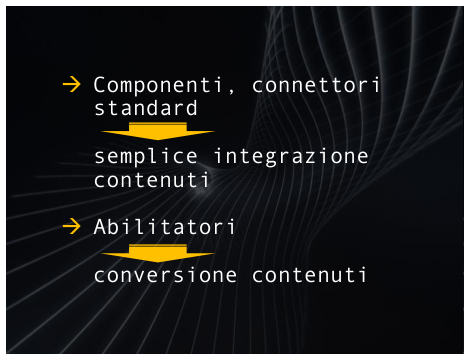
\includegraphics[width=0.50\textwidth,
                    trim=40 60 40 60, % L B R T
                    clip]
                    {images/Lez13_p04_fig_01}
  % \caption{Sommario}
  % \label{fig:Lez15_p06_fig_02}
\end{figure}
\FloatBarrier
\noindent

Richiedono l'utilizzo di componenti, connettori standard per collegare i vari contenuti acceduti perché una necessità è l'integrazione semplice dei vari contenuti.

Ma se da una parte questi applicativi di mashup facilitano l'integrazione dei dati, da un'altra parte non sono ancora stati definiti standard, definiti strumenti per l'integrazione, per il mashup di dati differenti, indipendentemente da qualsiasi formato loro di archiviazione.

Sono stati definiti degli abilitatori per la conversione dei contenuti.
Non si è puntato tanto alla standardizzazione dei formati o alla costruzione di funzioni di integrazione dei contenuti indipendentemente dal formato, ma alla traduzione di molti di questi formati per permettere una integrazione dei formati trasformati, dei formati diffusi in forma gestibile dai mashup, dagli applicativi specifici.

\subsection{Business Process as a Service}

\FloatBarrier
\begin{figure}[H]
  \centering
  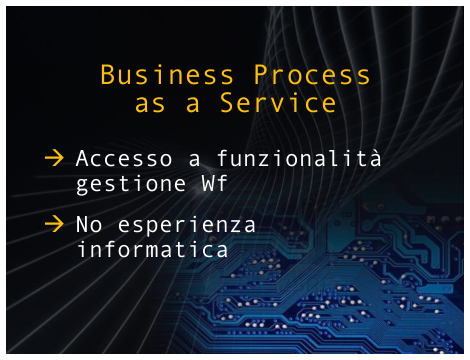
\includegraphics[width=0.50\textwidth,
                    trim=40 80 40 40, % L B R T
                    clip]
                    {images/Lez13_p04_fig_02}
  % \caption{Sommario}
  % \label{fig:Lez15_p06_fig_02}
\end{figure}
\FloatBarrier
\noindent

Il modello di servizio successivo è il Business Process as a Service.
Permette l'accesso a funzionalità gestionali, per esempio, alla gestione dei workflow.
La gestione dei workflow è una delle attività molto rilevanti dei sistemi informativi aziendali.
Possono essere definiti servizi di business process che forniscano accesso ad altri tipi di servizi per la gestione dell'organizzazione aziendale.
Rilevante è che l'accesso a questo tipo di servizi non richieda una particolare esperienza informatica.

\subsection{Network as a Service}

\FloatBarrier
\begin{figure}[H]
  \centering
  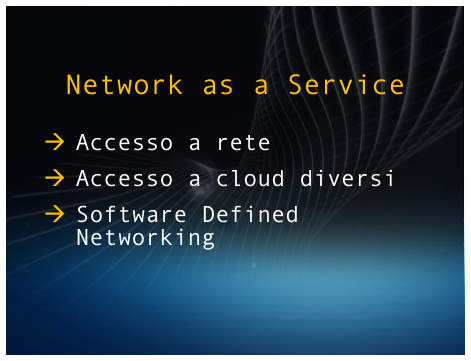
\includegraphics[width=0.50\textwidth,
                    trim=40 80 40 40, % L B R T
                    clip]
                    {images/Lez13_p04_fig_03}
  % \caption{Sommario}
  % \label{fig:Lez15_p06_fig_02}
\end{figure}
\FloatBarrier
\noindent

L'accesso alla rete può essere inteso come la fornitura di servizio di accesso generico alla rete, oppure anche l'accesso a un cloud diverso per necessità, ad esempio, di integrarsi con cloud complementari che offrano tipi di servizi o risorse non disponibili.

Questo modello di servizio è basato sul concetto software defined network.

\subsection{Network as a Service}

\FloatBarrier
\begin{figure}[H]
  \centering
  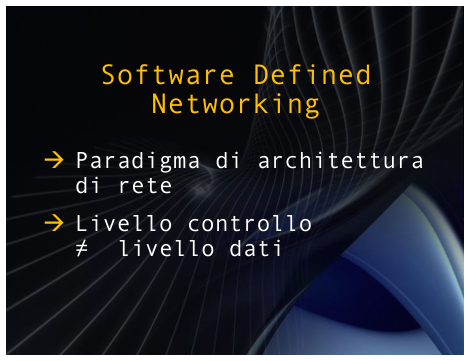
\includegraphics[width=0.50\textwidth,
                    trim=40 80 40 40, % L B R T
                    clip]
                    {images/Lez13_p04_fig_04}
  % \caption{Sommario}
  % \label{fig:Lez15_p06_fig_02}
\end{figure}
\FloatBarrier
\noindent

Software defined network è un paradigma di architettura di rete, un modello per organizzare la gestione della rete che è basato su un punto fondamentale.
Il livello di controllo, il livello di gestione della rete è separato dal livello dei dati.
Questo permette una gestione del servizio di rete più dinamico e più potente.

\FloatBarrier
\begin{figure}[H]
  \centering
  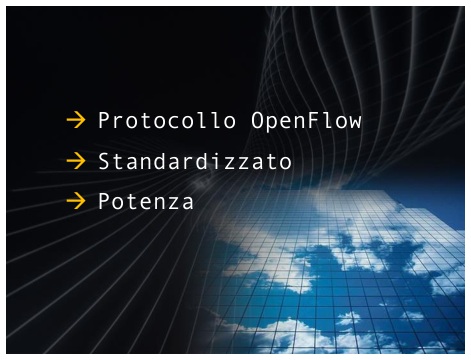
\includegraphics[width=0.50\textwidth,
                    trim=40 120 40 80, % L B R T
                    clip]
                    {images/Lez13_p04_fig_05}
  % \caption{Sommario}
  % \label{fig:Lez15_p06_fig_02}
\end{figure}
\FloatBarrier
\noindent

È basato innanzitutto sul protocollo OpenFlow che è stato presentato dall'Open Networking Foundation statunitense nel febbraio del 2011.
E' un metodo di gestione della rete standardizzato che permette una potenza notevole.
Questa separazione della gestione della parte fisica di dati dalla parte di controllo o gestionale permette di presentare all'utente una potenza, una quantità di risorse superiore a quella di fatto fisicamente disponibile.

\FloatBarrier
\begin{figure}[H]
  \centering
  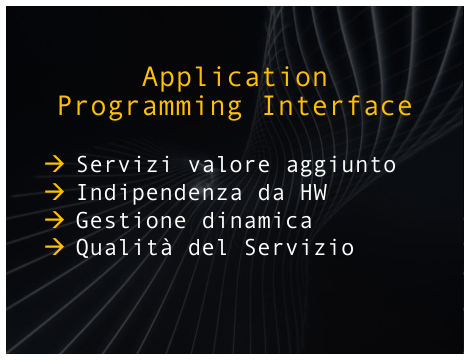
\includegraphics[width=0.50\textwidth,
                    trim=40 80 40 60, % L B R T
                    clip]
                    {images/Lez13_p04_fig_06}
  % \caption{Sommario}
  % \label{fig:Lez15_p06_fig_02}
\end{figure}
\FloatBarrier
\noindent

Per la gestione opportuna di questa separazione concettuale tra gestione dei dati e gestione del controllo viene fatto uso di Application Programming Interface per integrare servizi di valore aggiunto, per gestire l'indipendenza dall'hardware, quindi presentare una visione virtualizzata dell'accesso alla rete.

Le risorse di rete sono presentate, sono utilizzabili in una versione immagine che può avere dimensione o una potenza virtuale, una larghezza di banda nel caso della trasmissione di dati superiore a quella effettiva.

La gestione è dinamica e soprattutto la qualità del servizio risulta essere superiore.

Ricordiamo che nel caso del cloud computing la continuità e la qualità, l'efficacia, l'efficienza del servizio sono degli elementi basilari per il successo di questo modello.
%%%%%%%%%%%%%%%%%%%%%%%%%%%%29:31%%%%%%%%%%%%%%%%%%%%%%%%%%%%%%%%%%%
Spunti di riflessione: innanzitutto pensate che servizi informativi usate nella vostra attività lavorativa o formativa, provate a definire tutti gli elementi del sistema informativo o anche parzialmente.
Se fossero basati sul modello cloud, quale tipo di servizio sarebbe impiegato?

\section{Classi di consumatori}

\FloatBarrier
\begin{figure}[H]
  \centering
  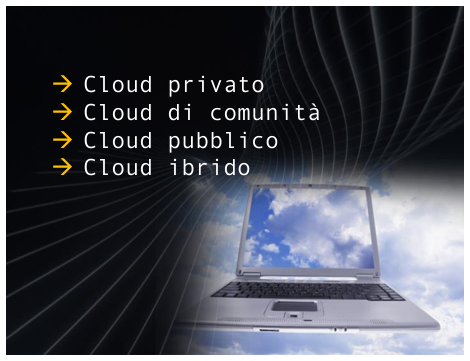
\includegraphics[width=0.50\textwidth,
                    trim=40 160 40 60, % L B R T
                    clip]
                    {images/Lez13_p05_fig_04}
  % \caption{Sommario}
  % \label{fig:Lez15_p06_fig_02}
\end{figure}
\FloatBarrier
\noindent

Sono individuate 4 classi.

Il cloud privato è utilizzato da un'organizzazione che ha un'utenza compatta che ha uno scopo condiviso e un sistema di gestione comune.

Cloud di comunità in cui possono partecipare più organizzazioni, più gruppi, quindi faremo riferimento a una collettività di utenti che abbiano degli scopi condivisi o quantomeno accordati.

Il cloud pubblico che può essere utilizzato da una varietà di utenti senza necessariamente raggruppamenti o specificità.

Il cloud in ibrido che è naturalmente definito come una moltepicità di sistemi di gestione del tipo precedente.

\subsection{Cloud Privato}

\FloatBarrier
\begin{figure}[H]
  \centering
  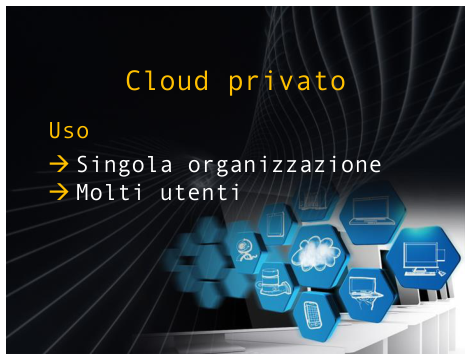
\includegraphics[width=0.50\textwidth,
                    trim=40 140 40 60, % L B R T
                    clip]
                    {images/Lez13_p05_fig_05}
  % \caption{Sommario}
  % \label{fig:Lez15_p06_fig_02}
\end{figure}
\FloatBarrier
\noindent

È utilizzato da una singola organizzazione ma molti utenti; un gruppo molteplice di utenti, può anche essere vasto, ma che abbiano un connettivo, lo scopo e il management.

\FloatBarrier
\begin{figure}[H]
  \centering
  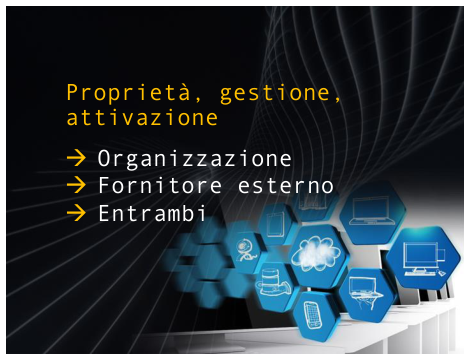
\includegraphics[width=0.50\textwidth,
                    trim=40 120 40 60, % L B R T
                    clip]
                    {images/Lez13_p05_fig_06}
  % \caption{Sommario}
  % \label{fig:Lez15_p06_fig_02}
\end{figure}
\FloatBarrier
\noindent

La proprietà, la gestione e l'attivazione possono essere o dell'organizzazione stessa, quindi della classe di utenza che abbiamo individuato come privata, oppure anche da un fornitore esterno; quindi essere data in outsourcing ma i rapporti con il fornitore gestiti dall'organizzazione stessa; oppure anche da entrambi, da una combinazione, la gestione di parte del sistema può essere affidata all'organizzazione interna, per esempio l'amministrazione, mentre la parte sistemistica, la parte tecnica di gestione delle risorse può essere affidata a un fornitore esterno.

\FloatBarrier
\begin{figure}[H]
  \centering
  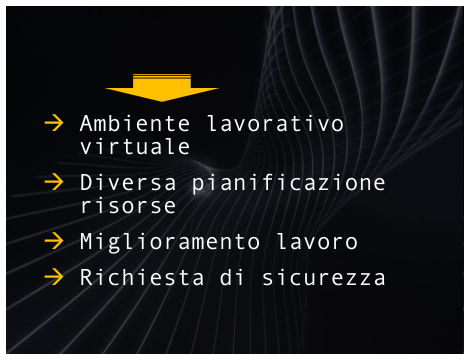
\includegraphics[width=0.50\textwidth,
                    trim=40 40 40 60, % L B R T
                    clip]
                    {images/Lez13_p06_fig_01}
  % \caption{Sommario}
  % \label{fig:Lez15_p06_fig_02}
\end{figure}
\FloatBarrier
\noindent

Adottare un cloud privato richiede un grande impegno perché l'ambiente lavorativo virtuale offre una nuova sfida organizzativa, sia se ci poniamo come gestori delle risorse, quindi in qualche modo offriamo, seppur a utenti all'interno della nostra organizzazione le risorse virtualizzate, sia se ci poniamo semplicemente come utenti.

Abbiamo visto che ci abituiamo o iniziamo a lavorare in un ambito in cui le risorse sono illimitate, ma d'altra parte il controllo di queste risorse è intermediato da gestori.
Non siamo più i diretti, secondo il modello, controllori della risorsa.
Non stiamo più lavorando sul nostro calcolatore fisico, ma stiamo lavorando su un calcolatore alocalizzato, su una risorsa fisica alocalizzata con l'intermediazione di una virtualizzazione, però avremo a disposizione la quantità di risorse che ci è necessaria.

La diversa pianificazione delle risorse fa parte di questa sfida.
L'organizzazione si abituerà alla pianificazione, all'utilizzo delle risorse in maniera differente da quella tradizionale; queste variazioni portano a un miglioramento del lavoro, perché il lavoro è più economico e non abbiamo limiti di risorse.
Possiamo utilizzare il tipo di servizio che più ci aggrada, che è più consono alle nostre esigenze.
Application as a service, piuttosto che platform as a service per lo sviluppo, piuttosto che infrastructure as a service se vogliamo costruire in un ambiente virtuale un nostro nuovo sistema di calcolo.

La richiesta di sicurezza è molto alta, dovuta all'intermediazione, non siamo più noi a controllare direttamente il sistema di calcolo fisico e software, dall'altra perché l'intermediazione della virtualizzazione offre più entrate a possibili malintenzionati che vogliano violare la sicurezza o la privacy del nostro ambiente.

\subsection{Cloud di Comunità}

\FloatBarrier
\begin{figure}[H]
  \centering
  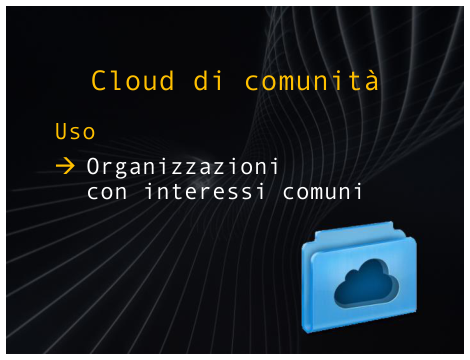
\includegraphics[width=0.50\textwidth,
                    trim=40 120 40 60, % L B R T
                    clip]
                    {images/Lez13_p06_fig_02}
  % \caption{Sommario}
  % \label{fig:Lez15_p06_fig_02}
\end{figure}
\FloatBarrier
\noindent

Vediamo ora i cloud di comunità.
L'uso è indirizzato a organizzazioni che hanno interessi comuni, quindi gruppi eterogenei di privati i cui scopi abbiano delle caratteristiche che motivano un qualche coordinamento nell'utilizzo di queste risorse.

\FloatBarrier
\begin{figure}[H]
  \centering
  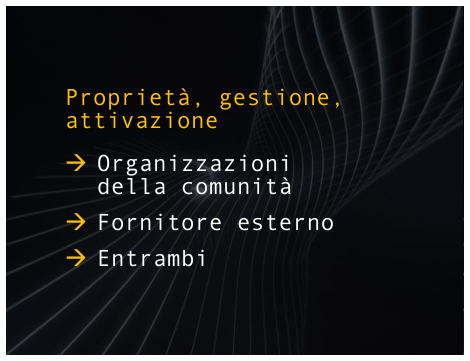
\includegraphics[width=0.50\textwidth,
                    trim=40 60 40 60, % L B R T
                    clip]
                    {images/Lez13_p06_fig_03}
  % \caption{Sommario}
  % \label{fig:Lez15_p06_fig_02}
\end{figure}
\FloatBarrier
\noindent

La proprietà, la gestione e l'attivazione può essere affidata ad alcune delle organizzazioni della comunità.
La comunità può comprendere un'organizzazione già dedicata al cloud computing, all'erogazione di servizi, eventualmente proprio per mantenere all'interno di questo consorzio di organismi la competenza per avere maggiore controllo nell'utilizzo di questo servizio.
Può essere affidato a un fornitore esterno, il gruppo, la federazione di privati, questa comunità non possiede le competenze e si rivolge a un fornitore esterno, oppure da entrambi.

\subsection{Cloud pubblico}

\FloatBarrier
\begin{figure}[H]
  \centering
  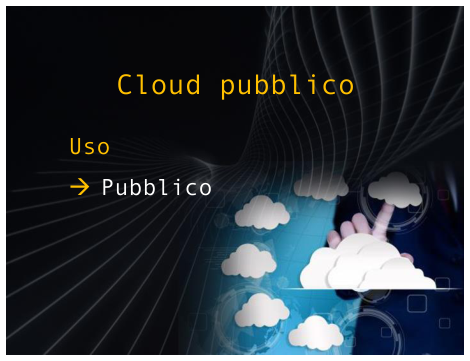
\includegraphics[width=0.50\textwidth,
                    trim=40 100 40 60, % L B R T
                    clip]
                    {images/Lez13_p06_fig_04}
  % \caption{Sommario}
  % \label{fig:Lez15_p06_fig_02}
\end{figure}
\FloatBarrier
\noindent

L'uso è rivolto al grande pubblico, gruppi illimitati come tipologia.

\FloatBarrier
\begin{figure}[H]
  \centering
  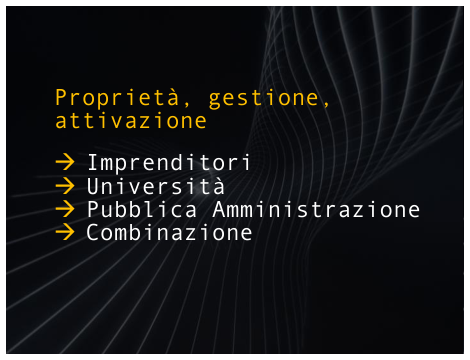
\includegraphics[width=0.50\textwidth,
                    trim=40 80 40 60, % L B R T
                    clip]
                    {images/Lez13_p06_fig_05}
  % \caption{Sommario}
  % \label{fig:Lez15_p06_fig_02}
\end{figure}
\FloatBarrier
\noindent

La proprietà, la gestione e l'attivazione può essere effettuata da imprenditori piuttosto che università, piuttosto che da pubblica amministrazione, naturalmente università o pubblica amministrazione, nel caso di gestione di risorse pubbliche che possono rivelarsi più adatte a questo tipo di classe di utenza piuttosto che anche da una combinazione dei tre principali precedenti, quindi un gruppo, una federazione composta da pubblica amministrazione, università pubblico-private o anche imprenditori.

\subsection{Cloud Ibrido}

\FloatBarrier
\begin{figure}[H]
  \centering
  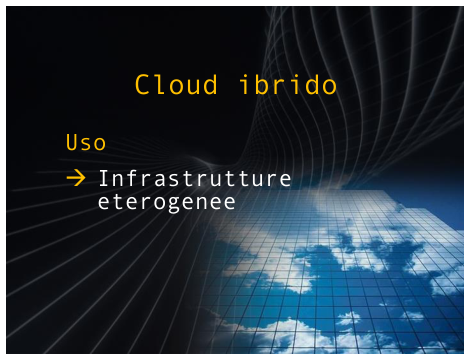
\includegraphics[width=0.50\textwidth,
                    trim=40 120 40 60, % L B R T
                    clip]
                    {images/Lez13_p06_fig_06}
  % \caption{Sommario}
  % \label{fig:Lez15_p06_fig_02}
\end{figure}
\FloatBarrier
\noindent

\FloatBarrier
\begin{figure}[H]
  \centering
  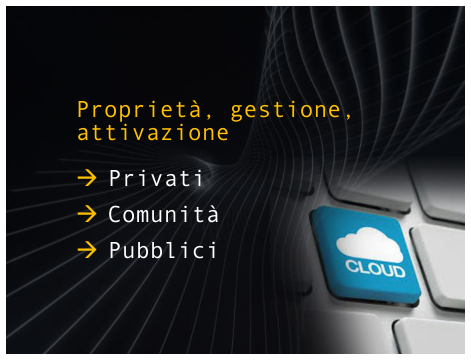
\includegraphics[width=0.50\textwidth,
                    trim=40 80 40 60, % L B R T
                    clip]
                    {images/Lez13_p07_fig_01}
  % \caption{Sommario}
  % \label{fig:Lez15_p06_fig_02}
\end{figure}
\FloatBarrier
\noindent

Il cloud ibrido è indirizzato a infrastrutture eterogene, quindi gestiti da privati piuttosto che da comunità di privati piuttosto che da organismi pubblici.

\FloatBarrier
\begin{figure}[H]
  \centering
  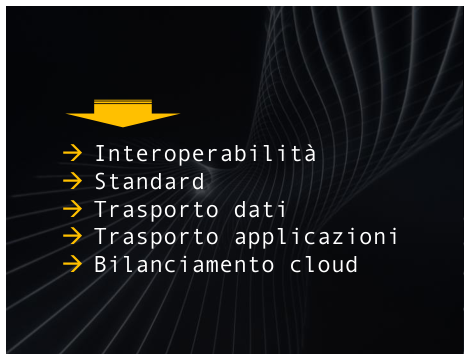
\includegraphics[width=0.50\textwidth,
                    trim=40 60 40 60, % L B R T
                    clip]
                    {images/Lez13_p07_fig_02}
  % \caption{Sommario}
  % \label{fig:Lez15_p06_fig_02}
\end{figure}
\FloatBarrier
\noindent

Cosa è importante però in questo caso?
A fronte della eterogenità dell'uso e della possibilità di gestione indirizzata a organismi molto differenti è necessario garantire l'interoperabilità tra i sistemi di gestione, tra le virtualizzazioni delle risorse, riferirsi a metodi, procedure standard, permettere il trasporto dei dati in qualunque e da qualunque locazione fisica o virtuale e attraverso qualunque risorsa, qualunque sistema di calcolo; deve permettere il trasporto, il trasferimento delle applicazioni da un cloud all'altro o da una risorsa all'altra e nel caso di cluster di cloud, permettere il bilanciamento del cloud, quindi permettere anche in qualche modo il controllo nell'uso delle risorse in un client e delle risorse dell'altro client.

Spunto di riflessione: in quale classe di consumatori inserireste la vostra realtà lavorativa e quella formativa? Privato, pubblico, ibrido? Argomentate.
